% Template: Fabian Wenzelmann, 2019, modified by us
\documentclass{beamer}

\usepackage[utf8]{inputenc}
\usepackage[ngerman]{babel} % use ngerman here for german text
\usepackage[T1]{fontenc}
\usepackage{mathtools}
\usepackage{amssymb}
\usepackage{lmodern}
\usepackage[protrusion=true,expansion=true,kerning]{microtype}
\usepackage{graphicx}
\usepackage{hyperref}
\usepackage{mdframed}
\usepackage{amsrefs}
\usepackage{bm}
\usepackage{amsmath}
\usepackage{movie15}
\usepackage{graphicx}
\DeclareMathOperator*{\argmin}{arg\,min}
\newtheorem{proposition}[theorem]{Proposition}
%\usepackage[center]{caption}

\usepackage{float}

%\usetheme{Pittsburgh}
%\usetheme{default}
\usetheme{Madrid}
%\usetheme{CambridgeUS}
%\usecolortheme{dolphin}
%\usecolortheme{dove}
%\usecolortheme{default}

%Bildunterschrift
%\addto\captionsngerman{%
%	\renewcommand{\figurename}{Abb.}%
%	\renewcommand{\tablename}{Tab.}%
%}

% einige Abkuerzungen
\newcommand{\qenc}{q_{\boldsymbol\phi}(\mathbf{z}|\mathbf{x}_i)}
\newcommand{\qencd}{q_{\phi}(z|x_i}
\newcommand{\penc}{p_{\boldsymbol\theta}(\mathbf{z}|\mathbf{x}_i)}
\newcommand{\pdec}{p_{\boldsymbol\theta}(\mathbf{x}_i|\mathbf{z})}
\newcommand{\C}{\mathbb{C}} % komplexe
\newcommand{\K}{\mathbb{K}} % komplexe
\newcommand{\R}{\mathbb{R}} % reelle
\newcommand{\Q}{\mathbb{Q}} % rationale
\newcommand{\Z}{\mathbb{Z}} % ganze
\newcommand{\N}{\mathbb{N}} % natuerliche
\newcommand{\E}{\mathbb{E}} % Erwartungswert
\newcommand{\F}{\mathcal{F}} 
\newcommand{\G}{\mathcal{G}} 


\newcommand{\tx}{\widetilde{x}}
\newcommand{\tz}{\widetilde{z}}
\newcommand{\tZ}{\widetilde{Z}}
\newcommand{\tX}{\widetilde{X}}
\newcommand{\tmu}{\widetilde{\mu}}
\newcommand{\tsig}{\widetilde{\sigma}}
\newcommand{\bP}{\mathbb{P}}
\newcommand{\bbf}{\bold{f}}
\newcommand{\bmu}{\bm{\mu}}
\newcommand{\bsig}{\bm{\sigma}}
\newcommand{\z}{\mathbf{z}}
\newcommand{\x}{\mathbf{x}_i}

\makeatletter
\newcommand{\vast}{\bBigg@{3}}
\newcommand{\Vast}{\bBigg@{5}}
\makeatother


\title[Hessian Free Optimization]{Efficient Hessian Free Optimization of Deep Neural Networks}
\subtitle{Niklas Brunn, No\"{e}l E. Kury, Clemens A. Schächter}

% For short you could for example use the last name only, it's optional as is
% the short title
\author[Numerical Optimization]{Project presentation at the Albert Ludwigs University of Freiburg\\
Numerical Optimization\\
Prof. Dr. Moritz Diehl\\
M.Sc. Florian Messerer}

%\date{11.02.22}

% removes the navigation symbols
% often they don't work and I find them rather annoying
\beamertemplatenavigationsymbolsempty{}

% You can have a logo to appear on all slides
 \logo{
\includegraphics[height=3.5cm]{Bilder/logo}}

\begin{document}
	
	\begin{frame}
		\titlepage
	\end{frame}
	
	
	
%\author[Clemens A. Schächter]{Nix}


\beamertemplatenavigationsymbolsempty{}

\logo{
\includegraphics[height=1cm]{Bilder/logo}}

\section{Experiments}   
\subsection{Simple simulated dataset}
\begin{frame}
\frametitle{Experiments: Simple simulated dataset}
\begin{itemize}
	\item[] 
\end{itemize}
\end{frame}
\subsection{MNIST}
\begin{frame}
\frametitle{Experiments: MNIST dataset}
\begin{itemize}
	\item[] 
\end{itemize}
\end{frame}




%\begin{frame}
%\frametitle{SDE Beispiele}
%\begin{tiny}SDE-Pfad-Simulationen von Ben Deitmar\end{tiny}
%\begin{figure}[h!]
%\begin{minipage}{0.4\textwidth}
%		%\begin{mdframed}[style=innersmall]
%		\center{}
%		\includegraphics[scale=0.27]{Bilder/SDE_sig=0}
%		\begin{tiny} $\mathrm{d}X_{t}=X_{t}\text{ }\mathrm{d}t+0\text{ }\mathrm{d}W_{t},$ $X_{0}=1$\\ $\mathrm{d}X_{t}=X_{t}\text{ }\mathrm{d}t+0\text{ }\circ \mathrm{d}W_{t},$ $X_{0}=1$ \end{tiny}
%		\center{}
%		\includegraphics[scale=0.27]{Bilder/SDE_BB}
%		\begin{tiny} $\mathrm{d}X_{t}=0\mathrm{d}t+\mathrm{d}W_{t},$ $X_{0}=1$\\ $\mathrm{d}X_{t}=0\mathrm{d}t+\circ\mathrm{d}W_{t},$ $X_{0}=1$\end{tiny}
%\center{}
%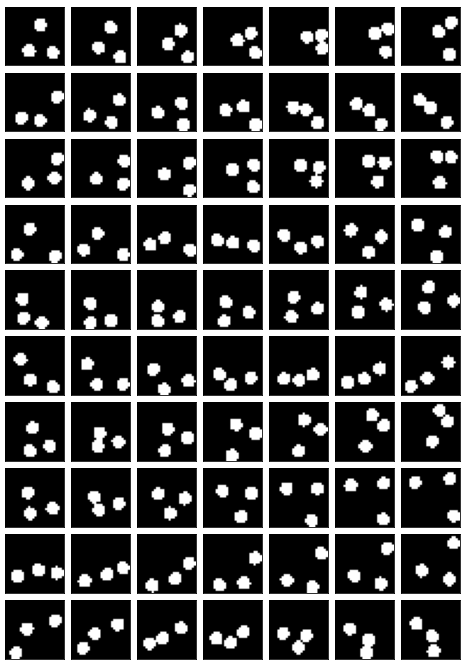
\includegraphics[scale=0.15]{Bilder/bouncingBalls_ODEorig2}
%\end{mdframed}
%	\end{minipage}
%\begin{minipage}{0.4\textwidth}
%\begin{mdframed}[style=innersmall]
%		\center{}
%		\includegraphics[scale=0.27]{Bilder/SDE_mu=x_sig=tt}
%		\begin{tiny} $dX_{t}=X_{t}\text{ }\mathrm{d}t+t^{2}\text{ }\mathrm{d}W_{t},$ $X_{0}=1$\\
%		$dX_{t}=X_{t}\text{ }\mathrm{d}t+t^{2}\text{ }\circ\mathrm{d}W_{t},$ $X_{0}=1$\end{tiny}
%\center{}
%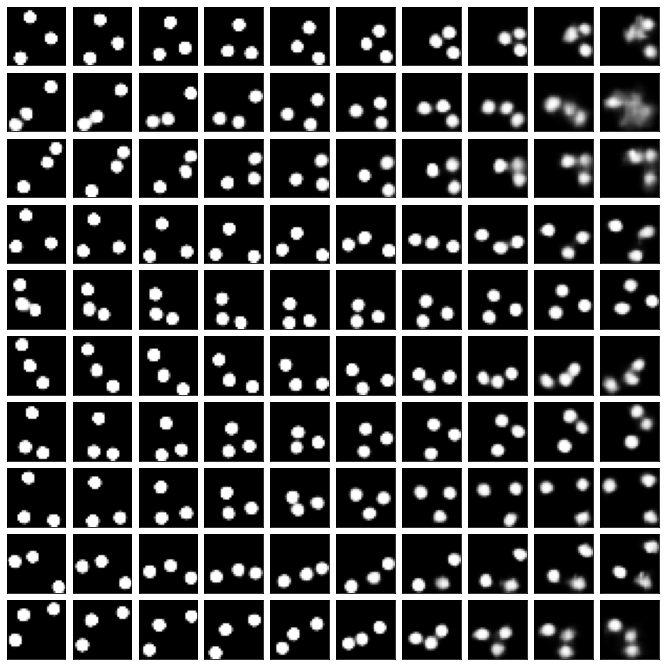
\includegraphics[scale=0.15]{Bilder/bouncingBalls_ODE}
%\end{mdframed}
%\end{minipage}
%\begin{minipage}{0.2\textwidth}
%\begin{mdframed}[style=innersmall]
%\center{}
%\includegraphics[scale=0.27]{Bilder/SDE_mu=x_sig=tt_x0=0}
%\begin{tiny} $dX_{t}=0+X_{t}\text{ }\mathrm{d}t+t^{2}\text{ }\mathrm{d}W_{t},$ $X_{0}=0$\\ $dX_{t}=0+X_{t}\text{ }\mathrm{d}t+t^{2}\text{ }\circ\mathrm{d}W_{t},$ $X_{0}=0$\end{tiny}
%\center{}
%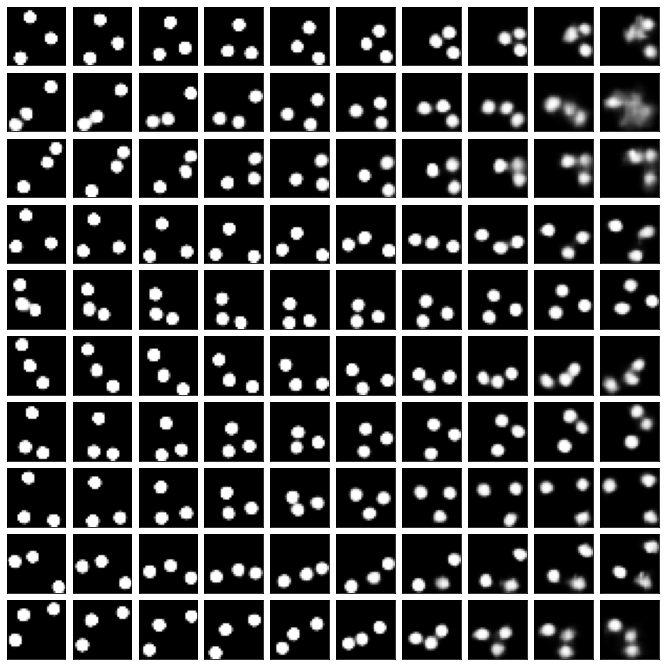
\includegraphics[scale=0.15]{Bilder/bouncingBalls_ODE}
%\end{mdframed}
% \end{minipage}
% \end{figure}
%\end{frame}

	
%\author[Clemens A. Schächter]{Nix}


\beamertemplatenavigationsymbolsempty{}

\logo{
\includegraphics[height=1cm]{Bilder/logo}}

\section{Experiments}   
\subsection{Simple simulated dataset}
\begin{frame}
\frametitle{Experiments: Simple simulated dataset}
\begin{itemize}
	\item[] 
\end{itemize}
\end{frame}
\subsection{MNIST}
\begin{frame}
\frametitle{Experiments: MNIST dataset}
\begin{itemize}
	\item[] 
\end{itemize}
\end{frame}




%\begin{frame}
%\frametitle{SDE Beispiele}
%\begin{tiny}SDE-Pfad-Simulationen von Ben Deitmar\end{tiny}
%\begin{figure}[h!]
%\begin{minipage}{0.4\textwidth}
%		%\begin{mdframed}[style=innersmall]
%		\center{}
%		\includegraphics[scale=0.27]{Bilder/SDE_sig=0}
%		\begin{tiny} $\mathrm{d}X_{t}=X_{t}\text{ }\mathrm{d}t+0\text{ }\mathrm{d}W_{t},$ $X_{0}=1$\\ $\mathrm{d}X_{t}=X_{t}\text{ }\mathrm{d}t+0\text{ }\circ \mathrm{d}W_{t},$ $X_{0}=1$ \end{tiny}
%		\center{}
%		\includegraphics[scale=0.27]{Bilder/SDE_BB}
%		\begin{tiny} $\mathrm{d}X_{t}=0\mathrm{d}t+\mathrm{d}W_{t},$ $X_{0}=1$\\ $\mathrm{d}X_{t}=0\mathrm{d}t+\circ\mathrm{d}W_{t},$ $X_{0}=1$\end{tiny}
%\center{}
%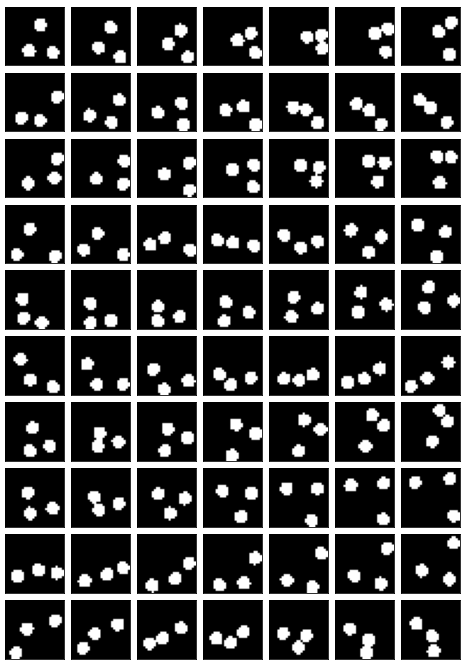
\includegraphics[scale=0.15]{Bilder/bouncingBalls_ODEorig2}
%\end{mdframed}
%	\end{minipage}
%\begin{minipage}{0.4\textwidth}
%\begin{mdframed}[style=innersmall]
%		\center{}
%		\includegraphics[scale=0.27]{Bilder/SDE_mu=x_sig=tt}
%		\begin{tiny} $dX_{t}=X_{t}\text{ }\mathrm{d}t+t^{2}\text{ }\mathrm{d}W_{t},$ $X_{0}=1$\\
%		$dX_{t}=X_{t}\text{ }\mathrm{d}t+t^{2}\text{ }\circ\mathrm{d}W_{t},$ $X_{0}=1$\end{tiny}
%\center{}
%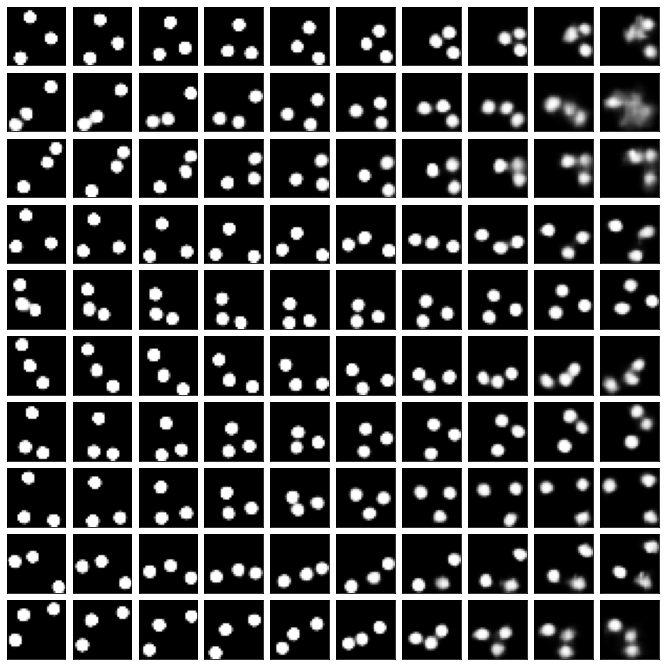
\includegraphics[scale=0.15]{Bilder/bouncingBalls_ODE}
%\end{mdframed}
%\end{minipage}
%\begin{minipage}{0.2\textwidth}
%\begin{mdframed}[style=innersmall]
%\center{}
%\includegraphics[scale=0.27]{Bilder/SDE_mu=x_sig=tt_x0=0}
%\begin{tiny} $dX_{t}=0+X_{t}\text{ }\mathrm{d}t+t^{2}\text{ }\mathrm{d}W_{t},$ $X_{0}=0$\\ $dX_{t}=0+X_{t}\text{ }\mathrm{d}t+t^{2}\text{ }\circ\mathrm{d}W_{t},$ $X_{0}=0$\end{tiny}
%\center{}
%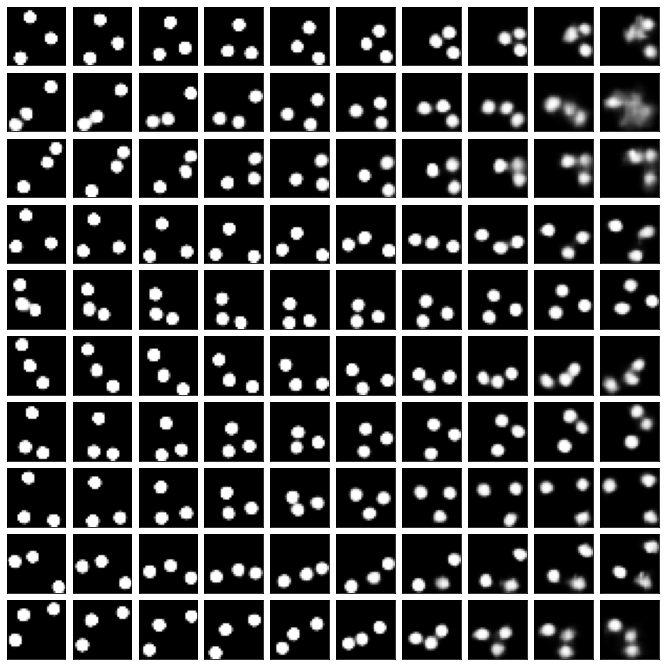
\includegraphics[scale=0.15]{Bilder/bouncingBalls_ODE}
%\end{mdframed}
% \end{minipage}
% \end{figure}
%\end{frame}

	
%\author[Clemens A. Schächter]{Nix}


\beamertemplatenavigationsymbolsempty{}

\logo{
\includegraphics[height=1cm]{Bilder/logo}}

\section{Experiments}   
\subsection{Simple simulated dataset}
\begin{frame}
\frametitle{Experiments: Simple simulated dataset}
\begin{itemize}
	\item[] 
\end{itemize}
\end{frame}
\subsection{MNIST}
\begin{frame}
\frametitle{Experiments: MNIST dataset}
\begin{itemize}
	\item[] 
\end{itemize}
\end{frame}




%\begin{frame}
%\frametitle{SDE Beispiele}
%\begin{tiny}SDE-Pfad-Simulationen von Ben Deitmar\end{tiny}
%\begin{figure}[h!]
%\begin{minipage}{0.4\textwidth}
%		%\begin{mdframed}[style=innersmall]
%		\center{}
%		\includegraphics[scale=0.27]{Bilder/SDE_sig=0}
%		\begin{tiny} $\mathrm{d}X_{t}=X_{t}\text{ }\mathrm{d}t+0\text{ }\mathrm{d}W_{t},$ $X_{0}=1$\\ $\mathrm{d}X_{t}=X_{t}\text{ }\mathrm{d}t+0\text{ }\circ \mathrm{d}W_{t},$ $X_{0}=1$ \end{tiny}
%		\center{}
%		\includegraphics[scale=0.27]{Bilder/SDE_BB}
%		\begin{tiny} $\mathrm{d}X_{t}=0\mathrm{d}t+\mathrm{d}W_{t},$ $X_{0}=1$\\ $\mathrm{d}X_{t}=0\mathrm{d}t+\circ\mathrm{d}W_{t},$ $X_{0}=1$\end{tiny}
%\center{}
%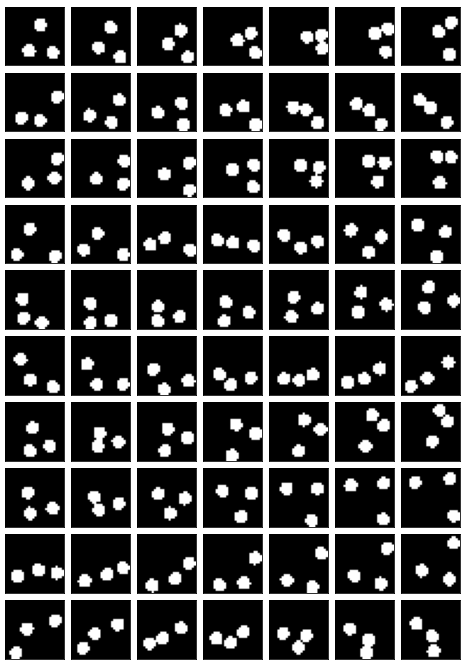
\includegraphics[scale=0.15]{Bilder/bouncingBalls_ODEorig2}
%\end{mdframed}
%	\end{minipage}
%\begin{minipage}{0.4\textwidth}
%\begin{mdframed}[style=innersmall]
%		\center{}
%		\includegraphics[scale=0.27]{Bilder/SDE_mu=x_sig=tt}
%		\begin{tiny} $dX_{t}=X_{t}\text{ }\mathrm{d}t+t^{2}\text{ }\mathrm{d}W_{t},$ $X_{0}=1$\\
%		$dX_{t}=X_{t}\text{ }\mathrm{d}t+t^{2}\text{ }\circ\mathrm{d}W_{t},$ $X_{0}=1$\end{tiny}
%\center{}
%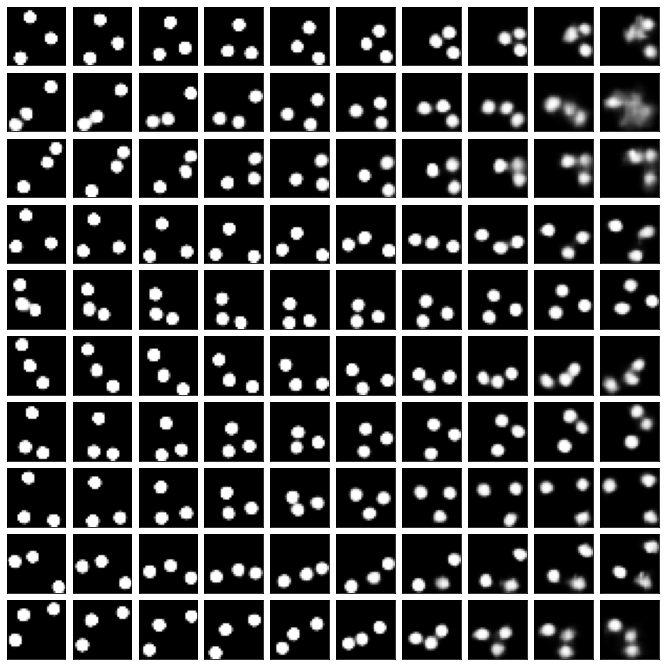
\includegraphics[scale=0.15]{Bilder/bouncingBalls_ODE}
%\end{mdframed}
%\end{minipage}
%\begin{minipage}{0.2\textwidth}
%\begin{mdframed}[style=innersmall]
%\center{}
%\includegraphics[scale=0.27]{Bilder/SDE_mu=x_sig=tt_x0=0}
%\begin{tiny} $dX_{t}=0+X_{t}\text{ }\mathrm{d}t+t^{2}\text{ }\mathrm{d}W_{t},$ $X_{0}=0$\\ $dX_{t}=0+X_{t}\text{ }\mathrm{d}t+t^{2}\text{ }\circ\mathrm{d}W_{t},$ $X_{0}=0$\end{tiny}
%\center{}
%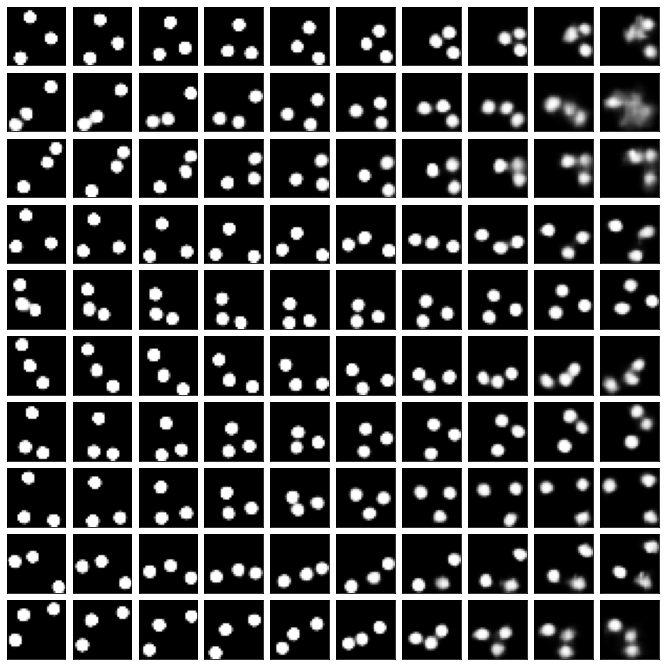
\includegraphics[scale=0.15]{Bilder/bouncingBalls_ODE}
%\end{mdframed}
% \end{minipage}
% \end{figure}
%\end{frame}



	\begin{frame}
		\frametitle{Sources}
		\begin{thebibliography}{9}
			
			\bibitem{b1} M. Diehl, "Lecture Notes on Numerical Optimization (Preliminary Draft)", Albert Ludwigs University of Freiburg, September 29, 2017	
			\bibitem{b2} M. Gargiani, A. Zanelli, M. Diehl, F. Hutter, "\text{}On the Promise of the Stochastic Generalized Gauss-Newton Method for Training DNNs",  arXiv:2006.02409v4, June 9, 2020 
			\bibitem{b3} J. Martens, "Deep learning via Hessian-free optimization", University of Toronto, Ontario, M5S 1A1, Canada, 2010
			\bibitem{b4} J. Martens, "New Insights and Perspectives on the Natural Gradient Method", Jurnal of Machine Learning Research 21, arXiv:1412.1193v11, September 19, 2020
			\bibitem{b5} J. Martens, I. Sutskever, "Training Deep and Recurrent Networks with Hessian-Free Optimization", In: G. Montavon, G.B. Orr, KR. Müller (eds), Neural Networks: Tricks of the Trade. Lecture Notes in Computer Science, vol 7700. Springer, Berlin, Heidelberg, 2012
			\bibitem{b6} N. N. Schraudolph, "Fast Curvature Matrix-Vector Products for Second-Order
			Gradient Descent", Neural Computation, August 2002
			
			
		\end{thebibliography}
	\end{frame}
	
\end{document}
